\documentclass[10pt]{article}
\usepackage{palatino}
\usepackage{fullpage}
\usepackage{latexsym}
\usepackage{amsfonts}
\usepackage{hyperref}
\usepackage{multicol}
\usepackage{fancyhdr}
\usepackage{enumitem}
\usepackage{caption}
\usepackage{subcaption}
\usepackage{fancybox}
\usepackage{framed}

\pagestyle{empty}                       %no page numbers
\thispagestyle{empty}                   %removes first page number
\setlength{\parindent}{0in}

\usepackage{fullpage}
\usepackage[tmargin = 0.5in, bmargin = 1in, hmargin = 1in]{geometry}     %1-inch margins
\geometry{letterpaper}
\usepackage{graphicx}
\usepackage{amssymb}

	\thispagestyle{empty}
	\renewcommand{\headrulewidth}{0.0pt}
	\thispagestyle{fancy}
	\lhead{Name: \underline{\hspace{1.5in}}}
	\chead{MTH 201: Calculus}
	\rhead{\framebox{\textbf{Grade: \ S \quad P}} }
	\lfoot{}
	\cfoot{}
	\rfoot{}


\begin{document}

	\vspace*{0in}

		\begin{center}
			\textbf{Learning Target C9} \\
			{Version 2} \\
		\end{center}

\begin{framed}
	\textbf{C9: Interpret areas under graphs as definite integrals, and use a graph of a function to compute a definite integral.
}
\end{framed}

Consider the function $f(x)$ defined on the interval $0 \leq x \leq 5$ given by the graph below. Each portion of the graph is either part of a line or part of a circle. 

\begin{center}
    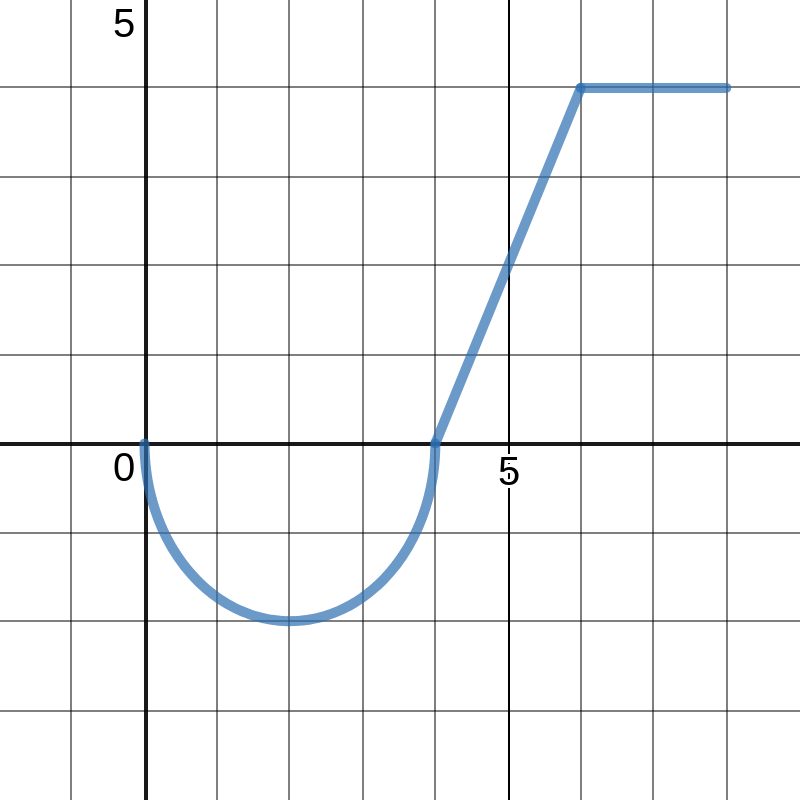
\includegraphics[width=3in]{c9-dec3.png}
\end{center}

Use known geometric formulas and the net signed area interpretation of the definite integral to evaluate each of the definite integrals below. You do not need to show your work, but see the Criteria for Satisfactory Work below. 

\begin{enumerate}
    \item $\displaystyle{\int_0^2 f(x) \, dx}$
    \item $\displaystyle{\int_4^8 f(x) \, dx}$
    \item $\displaystyle{\int_0^5 f(x) \, dx}$
\end{enumerate}


\vfill


\begin{small}
    \begin{framed}
        	\textbf{Criteria for Satisfactory grade:} At least two of the three integrals are correct. The third integral may contain errors that stem from careless mistakes in computation, \emph{not} including errors resulting from having incorrect signs on area values or mis-remembering geometry formulas. If the third integral is incorrect and there is no work shown, the grade will be Progressing. 
    \end{framed}
\end{small}

\end{document}
